% !TEX root = paper/paper.tex
\twocolumn[
\icmltitle{Dynamic Feature Selection for Classification on a Budget}

% It is OKAY to include author information, even for blind
% submissions: the style file will automatically remove it for you
% unless you've provided the [accepted] option to the icml2013
% package.
\icmlauthor{Sergey Karayev}{sergeyk@eecs.berkeley.edu}
\icmlauthor{Mario J. Fritz}{mfritz@mpi-inf.mpg.de}
\icmlauthor{Trevor Darrell}{trevor@eecs.berkeley.edu}

% You may provide any keywords that you
% find helpful for describing your paper; these are used to populate
% the "keywords" metadata in the PDF but will not be shown in the document
\icmlkeywords{test-time efficiency, feature selection, cost-sensitive, dynamic, mdp}

\vskip 0.3in
]

\section{Method}
{\itshape
The \textbf{test-time efficient classification problem} consists of
\vspace{-.5em}
\begin{itemize}
\addtolength{\itemsep}{-.55\baselineskip}
\item
$N$ instances labeled with one of $K$ labels: ${\mathcal{D} = \{x_n \in \mathcal{X}, y_n \in \mathcal{Y} = \{1, \dots, K\}\}_{n=1}^N}$.

\item
$F$ features $\mathcal{H} = \{h_f : \mathcal{X} \mapsto \mathbb{R}^{d_f} \}_{f=1}^F$, with associated costs $c_f$.

\item Budget-sensitive loss $\mathcal{L}_\mathcal{B}$, composed of cost budget $\mathcal{B}$ and loss function ${\ell(\hat{y}, y) \mapsto \mathbb{R}}$.
\end{itemize}

%\vspace{-.5em}
The goal is to find a \textbf{feature selection} policy $\pi(x): \mathcal{X} \mapsto 2^\mathcal{H}$ and a \textbf{feature combination} classifier $g(\mathcal{H}_\pi) : 2^\mathcal{H} \mapsto \mathcal{Y}$ such that such that the total budget-sensitive loss $\sum \mathcal{L}_\mathcal{B}(g(\pi(x_n)), y_n)$ is minimized.
}

The cost of a selected feature subset $\mathcal{H}_{\pi(x)}$ is $C_{\mathcal{H}_\pi(x)}$.
The budget-sensitive loss $\mathcal{L}_\mathcal{B}$ presents a \textbf{hard budget constraint} by only accepting answers with $C_{\mathcal{H}} \leq \mathcal{B}$.
Additionally, $\mathcal{L}_\mathcal{B}$ can be \textbf{cost-sensitive}: answers given with less cost are more valuable than costlier answers.
The motivation for the latter property is \textbf{\emph{Anytime}} performance; we should be able to stop our algorithm's execution at any time and have the best possible answer

\subsection{Feature selection as an MDP.}
{\itshape
The \textbf{feature selection MDP} consists of the tuple $(\mathcal{S}, \mathcal{A}, T(\cdot), R(\cdot), \gamma)$:
%\vspace{-.5em}
\begin{itemize}\addtolength{\itemsep}{-.55\baselineskip}
\item \textbf{State} $s \in \mathcal{S}$ stores the selected feature subset $\mathcal{H}_{\pi(x)}$ and their values and total cost $C_{\mathcal{H}_{\pi(x)}}$.
\item The set of \textbf{actions} $\mathcal{A}$ is the set of features $\mathcal{H}$.
\item The (stochastic) \textbf{state transition} distribution $T(s' \mid s, a)$ can depend on the instance $x$.
\item The \textbf{reward} function $R(s, a, s') \mapsto \mathbb{R}$ is manually specified, and depends on the classifier $g$ and the instance $x$.
\item The discount $\gamma$ determines amount of \textbf{lookahead} in selecting actions.
\end{itemize}
}

Reward definition is given in \autoref{fig:rewards}.

\vspace{1em}
\begin{figure}[h!]
    \centering
    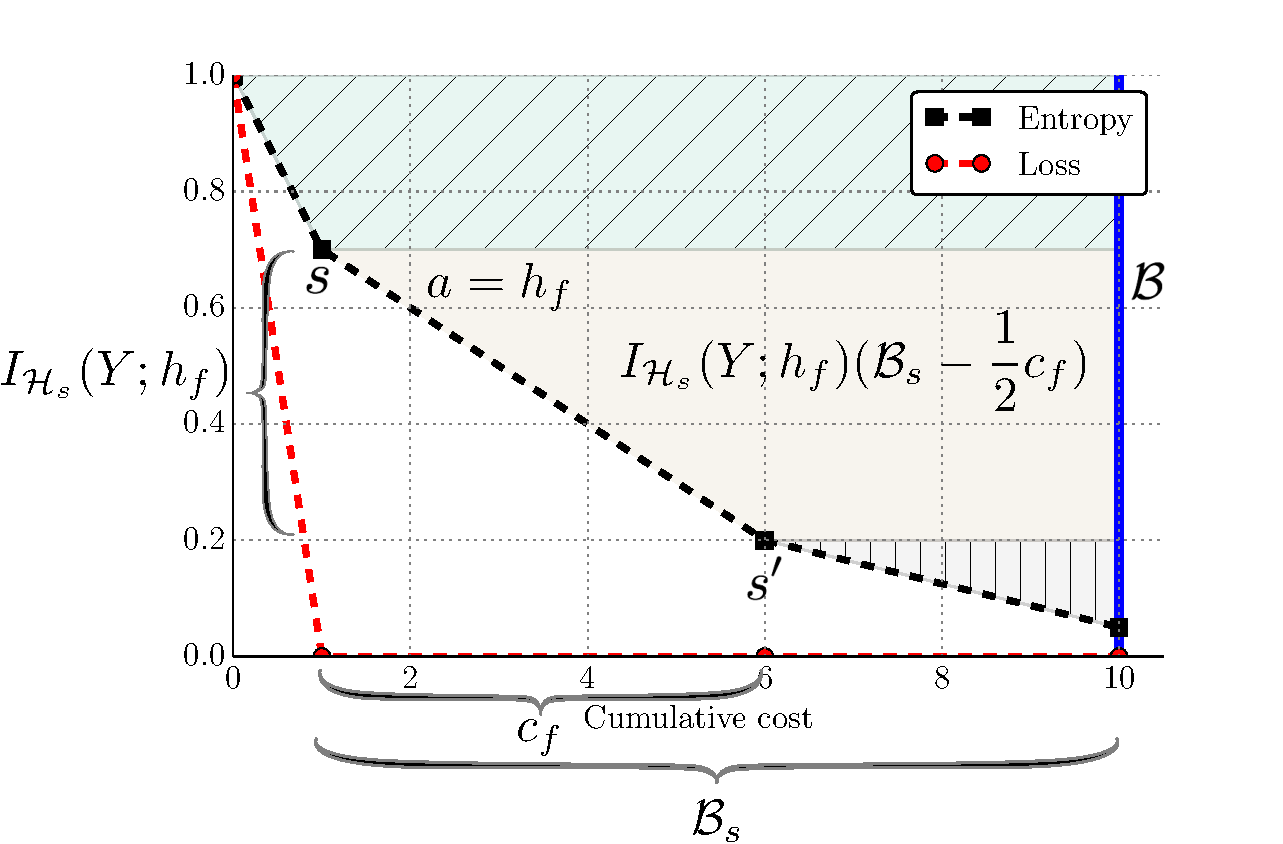
\includegraphics[width=\linewidth]{../../figures/rewards.pdf}
    \caption{
    Definition of the reward function.
    We seek to maximize the total area above the entropy vs. cost curve from $0$ to $\mathcal{B}$, and so define the reward of an individual action as the area of the slice of the total area that it contributes.
    From state $s$, action $h$ leads to state $s'$ with cost $c_f$.
    The information gain of the action $a = h_f$ is $I_{\mathcal{H}_s}(Y; h_f) = H(Y; \mathcal{H}_s) - H(Y; \mathcal{H}_s \cup {h_f})$.
    \label{fig:rewards}
    }


    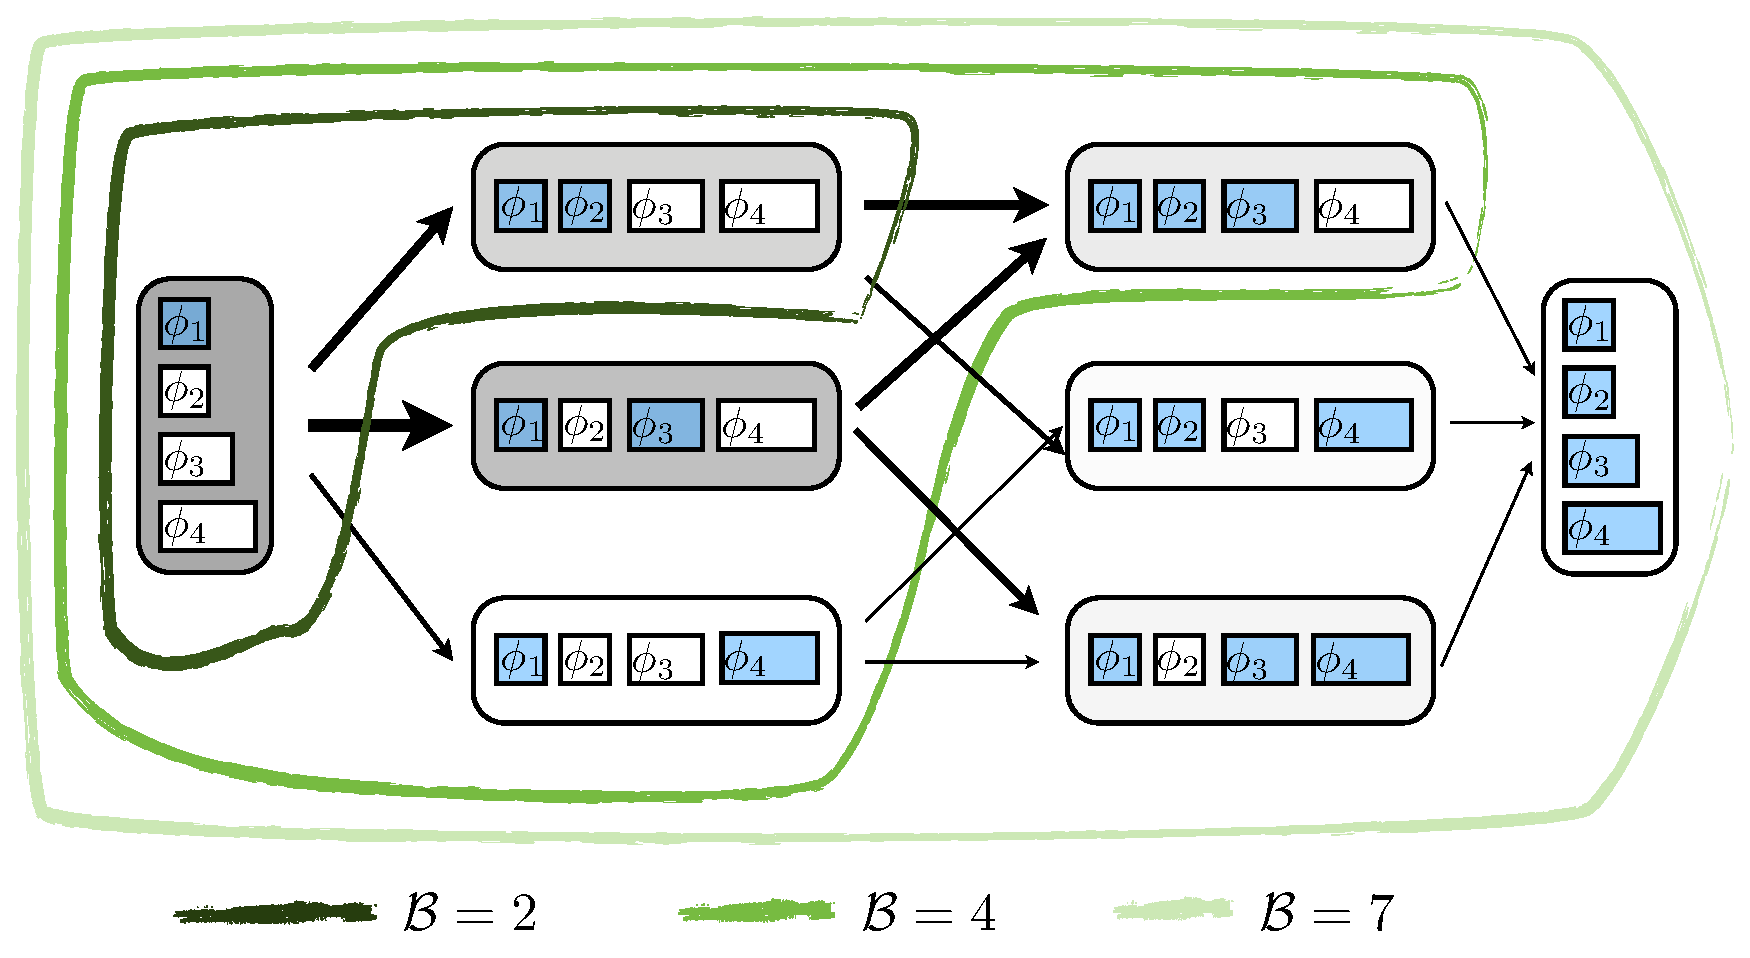
\includegraphics[width=.8\linewidth]{../../figures/mdp_masks.pdf}
    \caption{
    Illustration of the state space.
    The feature selection policy $\pi$ induces a distribution over feature subsets, for a dataset, which is represented by the shading of the larger boxes.
    Not all states are reachable for a given budget $\mathcal{B}$.
    We show three such ``budget cuts.''
    \label{fig:state_space}
    }
\end{figure}

\subsection{Learning the policy.}
We learn the state feature weight vector $\theta$ by \emph{policy iteration}.
First, we gather $(s, a, r, s')$ samples by running episodes with the current policy parameters $\theta_i$.
From these samples, $\hat{Q}(s, a)$ values are computed, and $\theta_{i+1}$ are given by $L_2$-regularized least squares solution to $\hat{Q}(s, a) = \theta^T \phi(s, a)$, on all states that we have seen in training.
During training, we gather samples starting from either a random feasible state, with decaying probability $\epsilon$, or from the initial empty state otherwise.

\subsection{Learning the classifier.}\label{sec:classifier}

A \textbf{Gaussian Naive Bayes} classifier can combine an arbitrary feature subset $\mathcal{H}_\pi$, but suffers from its restrictive generative model.
We found \textbf{logistic regression} to work better, but because it always uses the same length feature vector, unobserved feature values need to be imputed.
We evaluate \textbf{mean} and \textbf{Gaussian} imputation.

Since the classifier depends on the distribution over states (see Figure~\ref{fig:state_space}) induced by the policy, and the policy training depends on the entropy of the classifier, the learning procedure is iterative, alternating between learning policy and classifier.

Note that the policy $\pi$ selects some feature subsets more frequently than others.
Instead of learning only one classifier $g$ that must be robust to all observed feature subsets, we can learn several classifiers---for each of the most frequent subsets---and \textbf{match} test instances to classifier accordingly.

\section{Evaluation}
We evaluate the following baselines:
\vspace{-1em}
\begin{itemize}\addtolength{\itemsep}{-.55\baselineskip}
\item \textbf{Static, greedy}: corresponds to best performance of a policy that does not observe feature values and selects actions greedily ($\gamma=0$).
\item \textbf{Static, non-myopic}: policy that does not observe values but considers future action rewards ($\gamma=1$).
\item \textbf{Dynamic, greedy}: policy that observes feature values, but selects actions greedily.
\end{itemize}
\vspace{-1em}
Our method is the \textbf{Dynamic, non-myopic} policy: feature values are observed, with full lookahead.

\begin{figure}[h!]
\centering
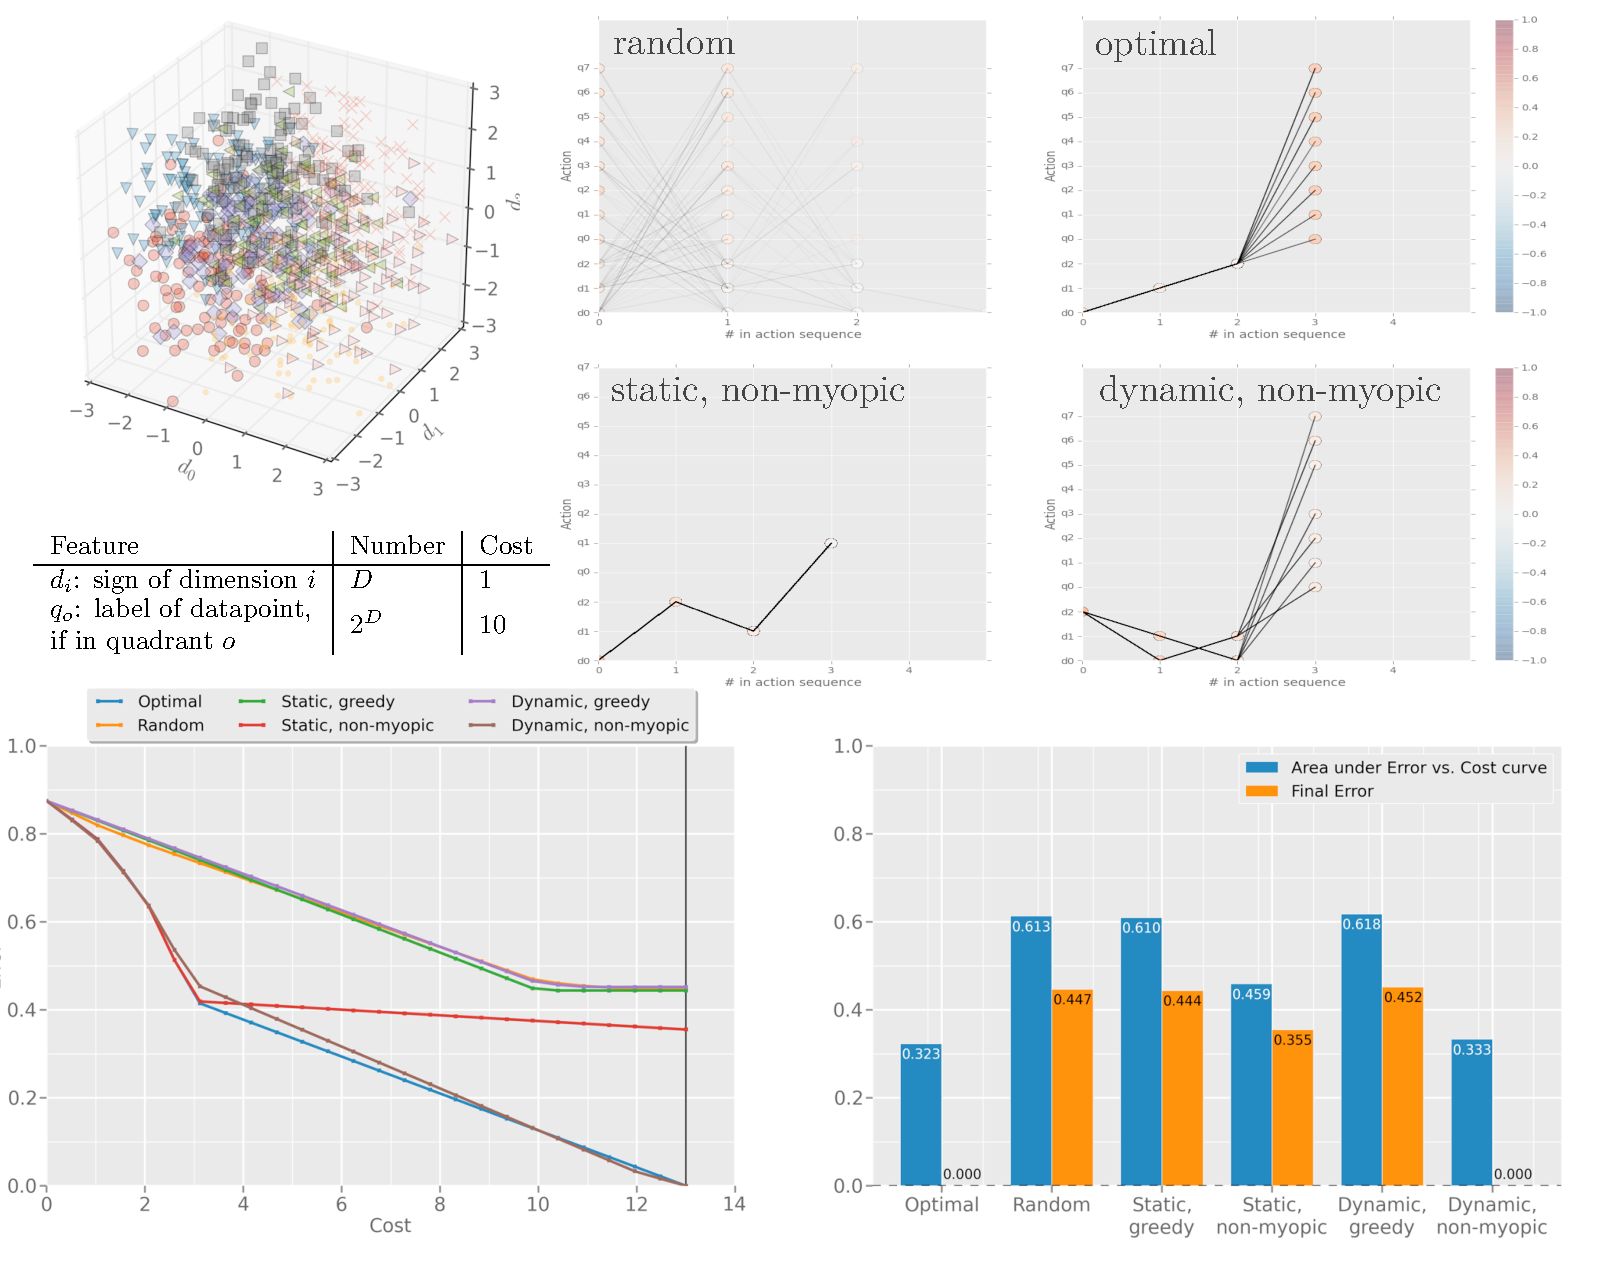
\includegraphics[width=\linewidth]{../../figures/synthetic_crop.pdf}
\vspace{-2em}
\caption{
Evaluation on the 3-dimensional synthetic example (best viewed in color).
The data is shown at top left; the sample feature trajectories of four different policies at top right.
The plots in the bottom half show that we recover the known optimal policy.
}
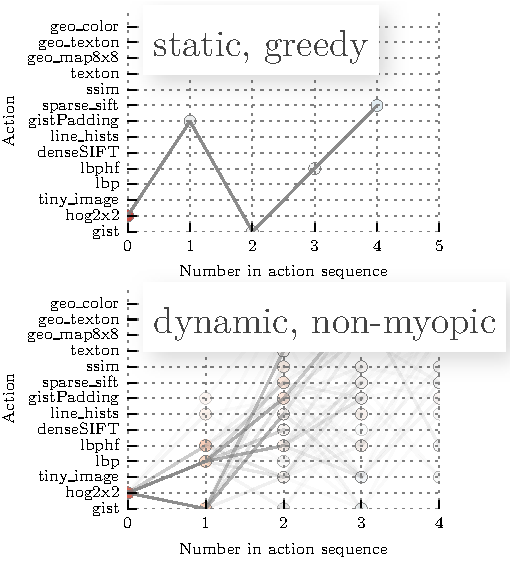
\includegraphics[width=\linewidth]{../../figures/scenes_result.pdf}
\caption{
Results on Scenes-15 dataset (best viewed in color).
14 visual features variy in cost from 0.3 to 8 seconds, and in accuracy from 0.32 to .82.
Our results on this dataset match the reported results of Active Classification \cite{Gao-NIPS-2011} and exceed the reported results of Greedy Miser \cite{Xu-ICML-2012}.
\label{fig:scenes}
}
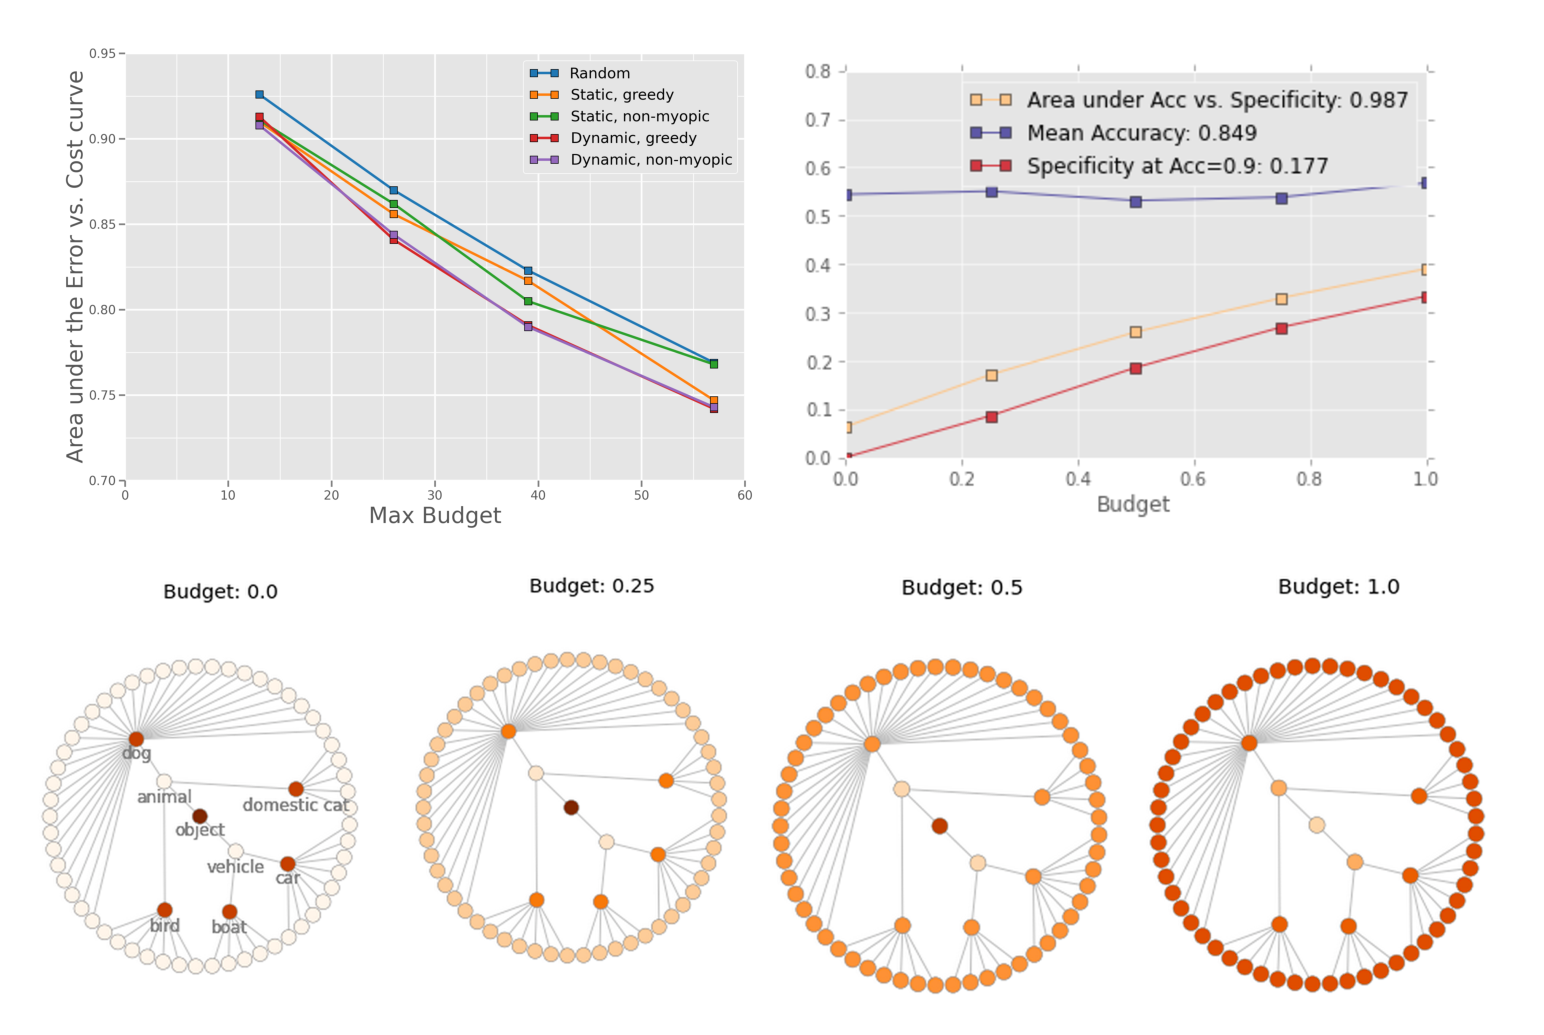
\includegraphics[width=\linewidth]{../../figures/imagenet}
\vspace{-1em}
\caption{
Results on the Imagenet 65-class subset. Note that when our method is combined with Hedging Your Bets \cite{Deng-CVPR-2012}, a constant accuracy can be achieved, with \emph{specificity} of predictions increasing with the budget, as in human visual perception.
(Color saturation corresponds to percentage of predictions at node.)
\label{fig:imagenet}}
\end{figure}

\bibliography{../../sergeyk_library}
\bibliographystyle{icml2013}
